\documentclass[11pt, a4paper, oneside]{exam}
\usepackage[margin=3cm]{geometry}
\usepackage{amsmath}
\usepackage{amsthm}
\usepackage{amsfonts}
\usepackage{MnSymbol}
\usepackage{appendix}
\usepackage{graphicx}
\usepackage{tikz}

\theoremstyle{definition}\newtheorem{define}{Definition}[section]
\theoremstyle{remark}\newtheorem{remark}{Remark}
\theoremstyle{definition}\newtheorem{example}{Example}[subsection]
\theoremstyle{definition}\newtheorem{notation}{Notation}[section]
\theoremstyle{definition}\newtheorem{theorem}{Theorem}[section]
\theoremstyle{definition}\newtheorem{corollary}{Corollary}[section]


\title{asdf}
\author{Name
}
\date{}

\begin{document}



% ------------------------------------------------------------------------------
%
% BODY PAGES
%
% ------------------------------------------------------------------------------

\section{Euclidean Vectors}

Informally speaking, vectors are mathematical objects that can be added together and multiplied by real numbers:

That is, if $\mathbf{v}, \mathbf{w}$ are vectors and $k$ is a real number, then
\begin{enumerate}
  \item $\mathbf{v} + \mathbf{w}$ is a vector.
  \item $k\mathbf{v}$ is a vector.
\end{enumerate}

Some examples of vectors: polynomials, real valued functions, sequences, arrows you can draw on the number plane, etc - we don't need to focus on most these from a vector perspective for the HSC.

The vectors of focus in the HSC course are those with \emph{direction} and \emph{length}, also known as Euclidean Vectors.

\begin{notation}[Component Form, Ordered Pairs, Column Notation]
	In two/three dimensional space, we define the following perpendicular, unit vectors (vectors with magnitude equal to 1):
	\begin{itemize}
		\item $\mathbf{i}$: the unit vector in the direction of the positive $x$-axis.
		\item $\mathbf{j}$: the unit vector in the direction of the positive $y$-axis.
		\item $\mathbf{k}$: the unit vector in the direction of the positive $z$-axis.
	\end{itemize}
	Note that in two dimensions, any linear combination of $\mathbf{i}$ and $\mathbf{j}$ and in three dimensions, any linear combination of $\mathbf{i}$, $\mathbf{j}$ and $\mathbf{k}$ can represent any vector in the space.

	Hence, the position $(a,b,c)$ can be represented by the following different notations:
	\begin{itemize}
    \item Component Form: $a\mathbf{i} + b\mathbf{j} + c \mathbf{k}$ - Also known as vector Quaternion form.
		\item Ordered Pair Form: $(a,b,c)$ - The components of the vectors are represented in the same way as the coordinate system.
    \item Column Notation: $\left[\begin{matrix} a \\ b \\ c\end{matrix}\right]$ - The components of the vectors are represented in a column.
  \end{itemize}
\end{notation}

\begin{notation}[Graphical Representation]
	Vectors in two/three dimensional space can be represented as directed line segments. The vector $\overrightarrow{AB}$ is represented by the tail end of the line segment at $A$, and the head at $B$:

	\begin{center}
		\begin{tikzpicture}
			\draw[fill = black,thick,->] (0,0) node [anchor = east] {$A$} -- (4,1) node [anchor = west] {$B$};
			\draw[fill = black] (0,0) circle (1pt);
		\end{tikzpicture}
	\end{center}
\end{notation}

	Any two vectors are equal if and only if they have equal magnitude and same direction. Hence, in a graphical representation, it does not matter where the directed line segment is drawn as long as it has the same length and direction as the vector that they represent. So, any graphical representation of a vector can be translated freely in the diagram.

\newpage
\section{Vector Addition and Scalar Multiplication}
In this part, we consider vector addition and scalar multiplication algebraically and geometrically.

\subsection{Scalar Multiplication}
For a vector $\vec{v} = \left[ \begin{matrix} v_1 \\ v_2 \end{matrix} \right]$ and $a \in \mathbb{R}$, $a\vec{v}$ is equal to $\left[ \begin{matrix} av_1 \\ av_2 \end{matrix} \right]$.

	Graphically, this is represented by the directed line segment of $\vec{v}$ lengthened by a factor of $a$.

\begin{example}$\empty$\\
	The vector $\mathbf{v} = 2\mathbf{i} + \mathbf{j}$ and $3\mathbf{v}$ is shown below:

	\begin{center}
		\begin{tikzpicture}
				\draw[->] (-2.5,0) -- (6.5,0) node[anchor = west] {$x$};
				\draw[->] (0,-2.5) -- (0,3.5) node[anchor = south] {$y$};
				\draw (0,0) node[anchor = north east] {$0$};
				\foreach \x in {-2,-1,1,2,...,6}
					\draw (\x,-0.1) node[anchor = north] {$\x$} -- (\x,0.1);
				\foreach \y in {-2,-1,1,2,3}
					\draw (-0.1,\y) node[anchor = east] {$\y$} -- (0.1,\y);

			\draw[->, thick] (0,0) -- (2,1);
			\draw[->] (0,0) -- (6,3);
		\end{tikzpicture}
	\end{center}
\end{example}

\subsection{Vector Addition}
\begin{align*}
	(a \mathbf{i} + b \mathbf{j}) + (c\mathbf{i} + d \mathbf{j}) & = (a \mathbf{i} + c \mathbf{i}) + (b \mathbf{j} + d\mathbf{j}) \\
	& = (a + c)\mathbf{i} + (b + d) \mathbf{j}
\end{align*}
Graphically, the vector sum is the diagonal of the parallelogram formed by translating the tail end of one vector to the other.

\begin{center}
	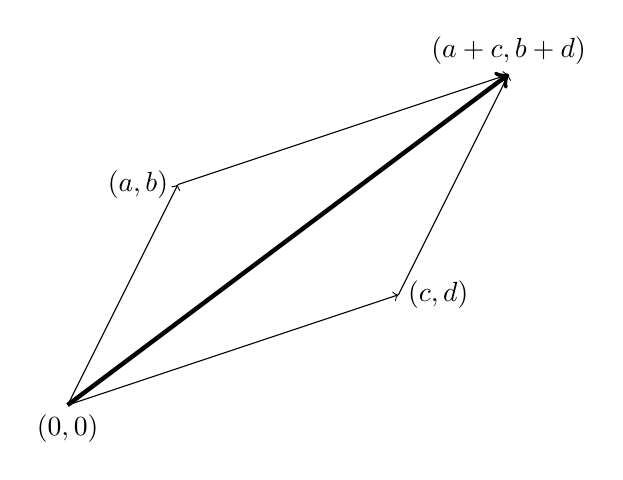
\begin{tikzpicture}[scale = 1.4]
		\draw[->] (0,0) node[anchor = north] {$(0,0)$} -- (1,2) node [anchor = east] {$(a,b)$};
		\draw[->] (0,0) -- (3,1) node [anchor = west] {$(c,d)$};
		\draw[->] (1,2) --++ (3,1) node [anchor = south] {$(a+c, b+d)$};
		\draw[->] (3,1) --++ (1,2);
		\draw[->,ultra thick] (0,0) -- (4,3);
	\end{tikzpicture}
\end{center}

\newpage
\subsection{Vector Subtraction}
Consider the position vectors $\mathbf{a}$ that represent the position $A = (1,3)$ and $\mathbf{b}$ represents the position $B = (4,1)$.

The algebraic representation of $\mathbf{b} - \mathbf{a}$ is equal to the \emph{displacement} vector \[\overrightarrow{AB} = (4-1,1-3) = (3,-2)\]

This can be represented graphically by translating the directed line segment so that the tail is on $A$ and the head is on $B$, and it is the off-diagonal of the parallelogram formed by the vectors:

\begin{center}
	\begin{tikzpicture}
		\draw[->] (-2.5,0) -- (6.5,0) node[anchor = west] {$x$};
		\draw[->] (0,-2.5) -- (0,3.5) node[anchor = south] {$y$};
		\draw (0,0) node[anchor = north east] {$0$};
		\foreach \x in {-2,-1,1,2,...,6}
			\draw (\x,-0.1) node[anchor = north] {$\x$} -- (\x,0.1);
		\foreach \y in {-2,-1,1,2,3}
			\draw (-0.1,\y) node[anchor = east] {$\y$} -- (0.1,\y);
		\draw[] (0,0) -- (1,3) node[anchor = east] {$\mathbf{a}$};
		\draw[] (0,0) -- (4,1) node[anchor = west] {$\mathbf{b}$};
		\draw[->,ultra thick] (1,3) -- (4,1);
	\end{tikzpicture}
\end{center}

Similarly, the geometric representation of $\mathbf{a} - \mathbf{b}$ is the displacement vector $\overrightarrow{BA}$.

\begin{center}
	\begin{tikzpicture}
		\draw[->] (-2.5,0) -- (6.5,0) node[anchor = west] {$x$};
		\draw[->] (0,-2.5) -- (0,3.5) node[anchor = south] {$y$};
		\draw (0,0) node[anchor = north east] {$0$};
		\foreach \x in {-2,-1,1,2,...,6}
			\draw (\x,-0.1) node[anchor = north] {$\x$} -- (\x,0.1);
		\foreach \y in {-2,-1,1,2,3}
			\draw (-0.1,\y) node[anchor = east] {$\y$} -- (0.1,\y);
		\draw[] (0,0) -- (1,3) node[anchor = east] {$\mathbf{a}$};
		\draw[] (0,0) -- (4,1) node[anchor = west] {$\mathbf{b}$};
		\draw[<-,ultra thick] (1,3) -- (4,1);
	\end{tikzpicture}
\end{center}

Hence:
\begin{itemize}
	\item Vector \emph{Addition} is represented by the diagonal of the parallelogram formed by the vectors.
	\item Vector \emph{Subtraction} is represented by the off-diagonal of the parallelogram formed by the vectors. Be careful with the direction of this vector.
\end{itemize}


\newpage
\section{Operations with Vectors}

In many textbooks, the dot product is usually defined first in terms of angles and lengths, which appeals to our natural intuition about objects with direction and length. However, it is actually the existence of the dot product that defines the notion of length and angles. So firstly we define the dot product of two vectors, and then see how length and angle is derived from this.

\begin{define}[Dot Product]$\empty$\\
	The dot product of two vectors $\mathbf{u} = (u_1,u_2,u_3)$ and $\mathbf{v} = (v_1,v_2,v_3)$ is defined as:
	\begin{equation*}
		\mathbf{u} \cdot \mathbf{v} = u_1v_1 + u_2v_2 + u_3 v_3
	\end{equation*}
\end{define}


\begin{define}[Length and Angle]$\empty$\\
\begin{itemize}
	\item The length of a vector is the square root of the dot product of the vector by itself. i.e.
		\[ |\mathbf{v}| = \sqrt{\mathbf{v}\cdot\mathbf{v}} \]
	\item The cosine of the angle of two unit vectors is equal to their dot product. i.e.
		\[ \cos \angle (\mathbf{u},\mathbf{v}) =  \frac{\mathbf{u}}{|\mathbf{u}|}\cdot \frac{\mathbf{v}}{|\mathbf{v}|}\]
\end{itemize}
\end{define}

\section{Parallel and Perpendicular Vectors}
\begin{define}[Parallel Vectors]$\empty$\\
	Two vectors $\mathbf{u}$ and $\mathbf{v}$ are parallel if and only if there exists a scalar $k \in \mathbb{R}$ such that:
	\[ \mathbf{u} = k\mathbf{v} \]
	i.e. they are scalar multiples of one another.
\end{define}

\begin{theorem}[Perpendicular Vectors]$\empty$\\
	Two vectors $\mathbf{u}$ and $\mathbf{v}$ are perpendicular if and only if $\mathbf{u} \cdot \mathbf{v} = 0$.
\end{theorem}
(Prove this!)

\section{Projections}
\fbox{\parbox{\textwidth}{
	\begin{define}[Projection of $\mathbf{u}$ onto $\mathbf{v}$]$\empty$\\
		The projection of a vector $\mathbf{u}$ onto another vector $\mathbf{v}$ is a function:
		\[ \mbox{proj}_{\mathbf{v}}(\mathbf{u}) \]
		such that:

		\begin{enumerate}
			\item The direction of $\mbox{proj}_{\mathbf{v}}(\mathbf{u})$ is in the same direction as $\mathbf{v}$.
			\item The magnitude of $\mbox{proj}_{\mathbf{v}}(\mathbf{u})$ is equal to $|\mathbf{u}|\cos\theta$ where $\theta$ is the angle between $\mathbf{u}$ and $\mathbf{v}$.
		\end{enumerate}

		Graphically, it is represented by the following diagram:

		\begin{center}
			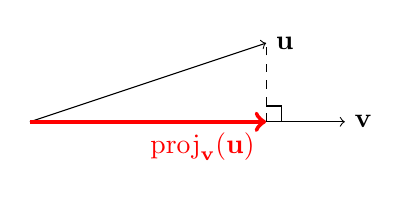
\begin{tikzpicture}
				\draw[->] (0,0) -- (4,0) node[anchor = west] {$\mathbf{v}$};
				\draw[->] (0,0) -- (3,1) node[anchor = west] {$\mathbf{u}$};
				\draw[->,ultra thick,red] (0,0) -- (3,0) node [anchor = north east] {$\mbox{proj}_\mathbf{v}(\mathbf{u})$};
				\draw[dashed] (3,0) -- (3,1);
				\draw[thin] (3.2,0) --++ (0,0.2) --++ (-0.2,0);
			\end{tikzpicture}
		\end{center}

		The formula for $\mbox{proj}_{\mathbf{v}}(\mathbf{u})$ is:
		\[ \mbox{proj}_{\mathbf{v}}(\mathbf{u}) = \left(\frac{\mathbf{u}\cdot \mathbf{v}}{\mathbf{v}\cdot \mathbf{v}}\right) \mathbf{v} \]



	\end{define}
}}
\begin{proof}
	The projection of $\mathbf{u}$ onto $\mathbf{v}$ can be constructed by multiplying its magnitude $|\mathbf{u}|\cos\theta$ onto the unit vector $\hat{\mathbf{v}}$:
	\begin{align*}
		\mbox{proj}_{\mathbf{v}}(\mathbf{u}) & = \left(|\mathbf{u}|\cos\theta \right) \hat{\mathbf{v}}\\
		& = \left(|\mathbf{u}|\cos\theta\right) \frac{\mathbf{v}}{|\mathbf{v}|}\\
		& = \left(\frac{|\mathbf{u}||\mathbf{v}|\cos\theta}{|\mathbf{v}|}\right) \frac{\mathbf{v}}{|\mathbf{v}|}\\
		& = \left(\frac{\mathbf{u}\cdot \mathbf{v}}{|\mathbf{v}|}\right) \frac{\mathbf{v}}{|\mathbf{v}|}\\
		& = \left( \frac{\mathbf{u}\cdot \mathbf{v}}{|\mathbf{v}|^2}\right) \mathbf{v}\\
    & = \left( \frac{\mathbf{u}\cdot \mathbf{v}}{\mathbf{v} \cdot \mathbf{v}}\right) \mathbf{v}
	\end{align*}
\end{proof}
\noindent Note: Learn the proof rather than the result! For Extension 2 students, see 2021 paper Q10 for why you should learn this proof.

\newpage
\section{Problem Set}

\begin{enumerate}
  \item Prove the following results about dot products:
  \begin{enumerate}
    \item $|\mathbf{a} + \mathbf{b}|^2 = |\mathbf{a}|^2 + 2 \mathbf{a}\cdot \mathbf{b} + |\mathbf{b}|^2$\\

    \item (Cauchy-Schwarz Inequality) $|\mathbf{u}\cdot \mathbf{v}| \leq |\mathbf{u}||\mathbf{v}|$\\

    \item (Triangle Inequality) $|\mathbf{u} + \mathbf{v}| \leq |\mathbf{u}| + |\mathbf{v}|$\\
  \end{enumerate}

  \item If $|\mathbf{a}| = 6$, $|\mathbf{b}| = 7$ and the angle between $\mathbf{a}$ and $\mathbf{b}$ is $60^\circ$, find:
  \begin{enumerate}
    \item $\mathbf{a} \cdot \mathbf{b}$\\
    \item $(\mathbf{a} + 2\mathbf{b})\cdot (3\mathbf{a} - \mathbf{b})$\\
    \item $|\mathbf{a} + \mathbf{b}|$\\
  \end{enumerate}

\item If $\mathbf{u}$, $\mathbf{v}$ and $\mathbf{u} + \mathbf{v}$ are unit vectors, find the angle between $\mathbf{u}$ and $\mathbf{v}$.\\

\item $\mathbf{a}, \mathbf{b},\mathbf{c}$ and $\mathbf{p}$ are vectors such that $\mathbf{a}\cdot \mathbf{c} =3$, $\mathbf{b}\cdot \mathbf{c} = 1$ and $\mathbf{p} = \mathbf{a} + k \mathbf{b}$. If $\mathbf{p}$ is perpendicular to $\mathbf{c}$, find the value of $k$.\\


\item In the figure below, $ABCD$ is a square with $\overrightarrow{AB} = \mathbf{i}$ and $\overrightarrow{AD} = \mathbf{j}$. $P$ and $Q$ are respectively points on $AB$ and $BC$ produced with $BP = k$ and $CQ = m$. $AQ$ and $DP$ intersect at $E$ and $\angle QEP = \theta$.

\begin{center}
	\begin{tikzpicture}[scale = 3]
		\draw[->] (0,0) node [anchor = north east] {$A$} -- (1,0) node [anchor = north] {$B$};
		\draw[->] (0,0) -- (0,1) node [anchor = east] {$D$};
		\draw (0,1) -- (1,1) node [anchor = west] {$C$} -- (1,0) -- (2.2,0) node[anchor = north west] {$P$} -- (0,1);
		\draw (0,0) -- (1,1.8) node [anchor = south] {$Q$} -- (1,0);
		\draw (0.455,0.798) node[anchor = north] {$E$};
		\draw (0.532, 0.85) node {$\theta$};
		\draw (0.5,0) node [anchor = north] {$\mathbf{i}$};
		\draw (0,0.5) node [anchor = east] {$\mathbf{j}$};
	\end{tikzpicture}
\end{center}

\begin{enumerate}
  \item By calculating $\overrightarrow{AQ} \cdot \overrightarrow{DP}$, find $\cos\theta$ in terms of $m$ and $k$.\\

	It is given that $\dfrac{DE}{EP} = \dfrac{1}{4}$.
  \item Express $\overrightarrow{AE}$ in terms of $k$.\\

  \item Let $\dfrac{AE}{AQ} = r$. Express $\overrightarrow{AE}$ in terms of $r$ and $m$.\\

  \item If $\theta = 90^\circ$, use the above results to find the values of $m$, $k$ and $r$.\\
  \end{enumerate}

\item $A$, $B$ and $C$ are points on a plane such that $\overrightarrow{OA} = 3 \mathbf{i} - \mathbf{j}$, $\overrightarrow{BC} = 7\mathbf{i} + \mathbf{j}$, and $\overrightarrow{OC} = x\mathbf{i} + y\mathbf{j}$, where $O$ is the origin.
\begin{enumerate}
  \item Find $\overrightarrow{CA}$, $\overrightarrow{OB}$ and $\overrightarrow{AB}$ in terms of $x$, $y$, $\mathbf{i}$ and $\mathbf{j}$.\\

  \item Given that $\overrightarrow{AB} \cdot \overrightarrow{BC} = 4 \overrightarrow{BC} \cdot \overrightarrow{CA}$, show that $y = 30 - 7x$.\\

  \item Furthermore, if $|\overrightarrow{BC}| = \sqrt{5}|\overrightarrow{CA}|$ and $x>0$, $y>0$,
	\begin{enumerate}
    \item find $x$ and $y$.\\
    \item show that $CA$ is perpendicular to $AB$.\\
    \item show that $O$ lies on $AB$.\\
	\end{enumerate}
\end{enumerate}

\item In the figure below, $\mathbf{x}$ and $\mathbf{y}$ are unit vectors, each of which makes an angle $\theta$ with the vector $\mathbf{z}$, where $\theta \in \left(0,\frac{\pi}{2}\right)$.

\begin{center}
	\begin{tikzpicture}
		\draw[->] (0,0) -- (3,0) node[anchor = west] {$\mathbf{x}$};
		\draw[->] (0,0) -- ({3*cos(70)},{3*sin(70)}) node[anchor = south] {$\mathbf{y}$};
		\draw[->] (0,0) -- ({3*cos(70) + 3},{3*sin(70)}) node[anchor = south west] {$\mathbf{z}$};
		\draw ({cos(17.5)},{sin(17.5)}) node {$\theta$};
		\draw ({cos(52.5)},{sin(52.5)}) node {$\theta$};
	\end{tikzpicture}
\end{center}
\begin{enumerate}
  \item Show that $\mathbf{x}\cdot \mathbf{z} = \mathbf{y}\cdot \mathbf{z}$.\\

  \item Let $\mathbf{z} = m\mathbf{x} + n\mathbf{y}$ for some constants $m$ and $n$. By expressing $\mathbf{x}\cdot\mathbf{z}$ and $\mathbf{y}\cdot\mathbf{z}$ in terms of $m$, $n$ and $\theta$, show that $m=n$.\\
\end{enumerate}

\item
A bug initially at the origin moves in a two-dimensional plane according to the velocity vector $\dfrac{d\mathbf{x}}{dt} = \left[ \begin{matrix}2\\3\end{matrix} \right]$ ms$^{-1}$.
\begin{enumerate}
  \item Calculate the speed of the bug.
  \item After two seconds, a gust of wind blows on the bug with velocity $\left[ \begin{matrix} -2\\1\end{matrix} \right]$ ms$^{-1}$ while the bug attempts to move with the same velocity.

  Find the position of the bug after another 3 seconds.
\end{enumerate}


\item Prove that the midpoints of the sides of a quadrilateral join to form a parallelogram.\\

\item Prove that the sum of the squares of the lengths of the diagonals of a parallelogram is equal to the sum of the squares of the lengths of the sides.\\

\item In a triangle $ABC$, $M$ and $N$ are the midpoints of $AB$ and $AC$ respectively. \\Prove that $MN \parallel BC$ and $MN = \dfrac{1}{2}BC$.

(Note: in the old HSC syllabus, students were required to memorise this result and the reason: ``line joining midpoints of two sides of a triangle is parallel to the third side and half its length".)\\

\item Prove that an angle in a semicircle is a right angle.\\

\item In a circle with centre $O$, $X$ is the midpoint of some chord $MN$. Prove that $OX \perp MN$.\\

\item In a quadrilateral $ABCD$, $M$ and $N$ are the midpoints of $AD$ and $BC$ respectively.\\
Show that $\overrightarrow{AB} + \overrightarrow{DC} = 2\overrightarrow{MN}$.\\

\item In a quadrilateral $ABCD$, $E$ and $F$ are the midpoints of $AB$ and $CD$ respectively. $G$ is the midpoint of $EF$.\\
Prove that $\overrightarrow{GA} + \overrightarrow{GB} + \overrightarrow{GC} + \overrightarrow{GD} = \mathbf{0}$.\\

\item
In the figure below, the lines $AB$ and $CD$ intersect at $O$. If $\dfrac{AO}{OB} = \dfrac{CO}{OD}$, prove by using vectors that $AC \parallel DB$.
\begin{center}
	\begin{tikzpicture}[scale=0.65]
		\draw ({5*cos(155)},{5*sin(155)}) node[anchor = south] {$A$} -- ({3*cos(-25)},{3*sin(-25)}) node[anchor = north] {$B$} -- ({4*cos(35)},{4*sin(35)}) node[anchor = south] {$D$} -- ({(20/3)*cos(215)},{(20/3)*sin(215)}) node[anchor = north] {$C$} -- cycle;
		\draw (0,0) node[anchor = north] {$O$};
	\end{tikzpicture}
\end{center}

\item In a parallelogram $ABCD$, $E$ and $F$ are two points on the diagonal $AC$ such that $AE = FC$.\\
Prove that $BFDE$ is a parallelogram.\\

\item Given two vectors $\mathbf{u} = \cos\theta \mathbf{i} + \sin\theta \mathbf{j}$ and $\mathbf{v} = \cos\phi \mathbf{i} + \sin\phi \mathbf{j}$, where $\theta > \phi$:
\begin{enumerate}
  \item Show that $\mathbf{u}$ and $\mathbf{v}$ are unit vectors.\\
  \item By considering the dot product, prove that $\cos(\theta - \phi) = \cos\theta \cos\phi + \sin\theta \sin\phi$.\\
\end{enumerate}

\item
In the standard coordinate system, the vector $\mathbf{v} = 3\mathbf{i} + 5\mathbf{j}$ means the vector $\mathbf{v}$ is the sum of 3 multiples of $\mathbf{i} = \left[ \begin{matrix} 1\\0\end{matrix} \right]$ and 5 multiples of $\mathbf{j} = \left[\begin{matrix} 0 \\ 1\end{matrix}\right]$. The position of this vector is given by the coordinate $(3,5)$ in this system.

Let the vectors $\mathbf{e_1} = 2\mathbf{i} + \mathbf{j}$ and $\mathbf{e_2} = -2\mathbf{i} + 4\mathbf{j}$.

We wish to form a new coordinate system with $\mathbf{e_1}$ and $\mathbf{e_2}$, i.e. vectors will be written in the form $a_1\mathbf{e_1} + a_2\mathbf{e_2}$ in this new coordinate system for some real constants $a_1$, $a_2$. In this new coordinate system, let the position of the vector be notated by $(a_1, a_2)^\prime$.

\begin{enumerate}
  \item Convert $(6,3)$ in the standard coordinate system to the new coordinate system given by $\mathbf{e_1}$ and $\mathbf{e_2}$.
  \item Convert $(13,37)$ in the standard coordinate system to the new coordinate system. (Hint: use the concept of vector projections.)
  \item Consider the vectors $\mathbf{v} = 2\mathbf{e_1} + 3\mathbf{e_2}$ and $\mathbf{w} = -5\mathbf{e_1} + 7\mathbf{e_2}$.

  Find $\mathbf{v}\cdot \mathbf{w}$.
\end{enumerate}





\end{enumerate}


% ------------------------------------------------------------------------------

\end{document}


